% a simple template with cesbio color code

\documentclass[xcolor=table, t]{beamer} 

\usepackage[utf8]{inputenc}
\usepackage{booktabs, comment} 
\usepackage[absolute, overlay]{textpos} 
\usepackage{pgfpages}
\usepackage{caption}
\usepackage[font=footnotesize]{caption}
\usepackage{multirow}
\usepackage{hyperref}
\usepackage{blindtext}
\usepackage{amsmath}
\usepackage[makeroom]{cancel}
\usepackage{textpos}
\usepackage{tikz}
\usepackage{csquotes}

\usepackage[T2A]{fontenc}
\usepackage[english, russian]{babel}

\setbeamertemplate{bibliography item}{\insertbiblabel}



% CESBIO ADAPTED COLOURS 
\definecolor{colorcesbio}{RGB}{37, 145, 17}
\definecolor{forestgreen}{rgb}{0.13, 0.55, 0.13}
\definecolor{greenyellow}{rgb}{0.68, 1.0, 0.18}
\definecolor{inchworm}{rgb}{0.7, 0.93, 0.36}

% MY COLOURS
\definecolor{agentP}{HTML}{1F8389}

% OPTIONAL COLOURS
% you can add the ones you need : lot of proposition on http://latexcolor.com/
\definecolor{ballblue}{rgb}{0.13, 0.67, 0.8}
\definecolor{chromeyellow}{rgb}{1.0, 0.65, 0.0}
\definecolor{darkcyan}{rgb}{0.0, 0.55, 0.55}
\definecolor{darkpastelred}{rgb}{0.76, 0.23, 0.13}
\definecolor{electricgreen}{rgb}{0.0, 1.0, 0.0}
\definecolor{electriclime}{rgb}{0.8, 1.0, 0.0}
\definecolor{deepcarrotorange}{rgb}{0.91, 0.41, 0.17}

% CESBIO ADAPTED BEAMER OPTIONS
\setbeamercolor{title in head/foot}{bg=inchworm, fg=forestgreen}
\setbeamercolor{author in head/foot}{bg=colorcesbio}
\setbeamertemplate{page number in head/foot}{}

\useoutertheme{infolines}
\usetheme{Madrid}
\usecolortheme[named=agentP]{structure}

% SPECIFIC COMMANDS
% if you nee to set command for youe presentation, you can put them here
\newcommand{\defnotation}[1]{\bf{\textsl{#1}}}

% BACKGROUND
\setbeamertemplate{background}
{
\includegraphics[width=\paperwidth,height=\paperheight]{BG.jpg}}

\hypersetup{
    colorlinks=true,
    linkcolor=ballblue,
    filecolor=magenta,      
    urlcolor=ballblue,
    pdfpagemode=FullScreen,
}



% PRESENTATION INFORMATIONS
% to fill in

\title[Шар]{Шар -- интересная геометрическая фигура}
\subtitle{Презентация}

\titlegraphic{
\includegraphics[height=2.0cm]{ВШЭ-round.png}}
\author[Никитин Д.Д.]{
	Никитин Д.Д. }
\institute[]{Факультет Компьютерных Наук \\ НИУ ВШЭ}
\date{Июль 2022}

% cesbio adapted frame structure
\setbeamercolor{navigation symbols}{bg=agentP, fg=agentP}
\addtobeamertemplate{navigation symbols}{}{%
    \usebeamerfont{footline}%
    \usebeamercolor[fg]{footline}%
    \hspace{1em}%
    \insertframenumber/\inserttotalframenumber
}

% Cover frame
\begin{document}
\begin{frame}
\maketitle
\end{frame}

% cesbio logo on all frames
\logo{
\includegraphics[height=1.7cm]{ВШЭ-round.png}~}


% Оглавление
\begin{frame}
\frametitle{Оглавление}
\tableofcontents
\end{frame}

% Определегние
\section{Определение шара}
\begin{frame}
    \frametitle<presentation>{Определение шара}
    % \framesubtitle{First elements of context}
    \begin{block}{Определение}
    \textit{Шар} -- геометрическое тело, ограниченное сферической или шаровой  поверхностью. Все нормали к поверхности сферы сходятся в центре шара, и все точки сферы отстоят на равных расстояниях от центра. \cite{dictionary1890efrona}
    \end{block}
    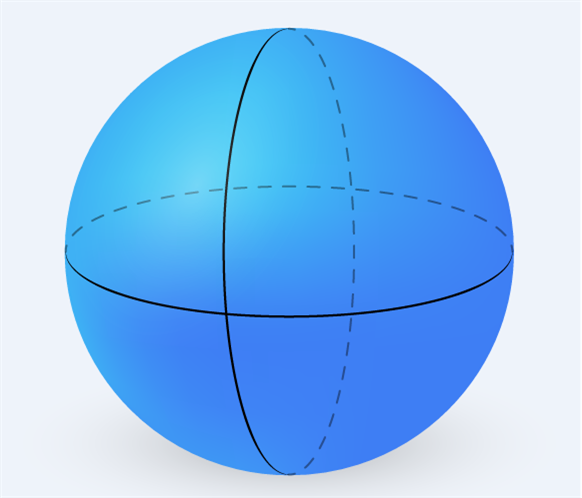
\includegraphics[width=0.4\textwidth]{Шар.png}
\end{frame}

% your section structure and all your frames

% Формулы
\section{Формулы}
\begin{frame}
    \frametitle<presentation>{Формулы}
    \textit{Формула объёма} n-мерного шара радиуса r в n-мерном евклидовом пространстве:
    $$ V_n(r)=\frac{\pi^\frac{n}{2}}{\Gamma(\frac{n}{2} + 1)}\cdot r^n, $$
    где $ \Gamma $ -- \href{https://univerlib.com/mathematical_analysis/parameter_integrals/euler_integrals/}{эйлеровская гамма-функция} \cite{olver2016nist}
    \newline
    \begin{flushleft}
    \begin{tabular}{ |p{3cm}|p{2cm}|p{2cm}|  }
        \hline
        \multicolumn{3}{|c|}{\textcolor{agentP}{Формулы для метрик шара}}\\
        \hline
        \textcolor{agentP}{Площадь, $ S $} & \textcolor{agentP}{$ 4\pi r^2 $} & \textcolor{agentP}{$ \pi d^2 $}\\[2ex]
        \hline
        \textcolor{agentP}{Объём, $ V $} & \textcolor{agentP}{$ \frac{4}{3} \pi r^3 $} & \textcolor{agentP}{$ \frac{\pi d^3}{6} $}\\[2ex]
        \hline
    \end{tabular}
    \end{flushleft}
    \href{https://onlinetestpad.com/ru/testview/696278-sfera-shar-ploshhad-sfery}{\beamerbutton{Для тех, кто хочет попрактиковаться, здесь лежит тест}}
\end{frame}

% Свойства шара
\section{Свойства шара}
\begin{frame}
    \frametitle<presentation>{Свойства шара}
    \begin{itemize}
        \item<1-> Любое сечение шара плоскостью есть круг.
        \item<3-> Через любые две точки, кроме \textit{диаметрально противоположных точек}, можно провести только один большой круг для шара.
        \item<5-> Если расстояние между центрами любых двух шаров меньше суммы их радиусов и больше модуля разности их радиусов, то такие шары \textbf{пересекаются}, а в плоскости пересечения образуется круг.
        \item<4-> Любые два больших круга одного шара пересекаются по прямой, проходящей через центр шара, а окружности пересекаются в двух \textit{диаметрально противоположных точках}.
        \item<2-> Через любые две \textit{диаметрально противоположные точки} можно провести множество больших кругов для шара.
    \end{itemize}
\end{frame}

% Литература
\section{Литература}
% [allowframebreaks]
\begin{frame}
        \frametitle<presentation>{Литература}
        \bibliographystyle{plain}
        \bibliography{bib_presentation.bib}
\end{frame}

\end{document}